\documentclass[a4paper, 10pt, final, garamond]{book}
\usepackage{cours-preambule}
\graphicspath{{./figures/}}

\makeatletter
\renewcommand{\@chapapp}{Contr\^ole de connaissances}
\makeatother

% \toggletrue{student}
% \toggletrue{corrige}
\renewcommand{\mycol}{black}
% \renewcommand{\mycol}{gray}

\begin{document}
\setcounter{chapter}{21}

\settype{enon}
\settype{solu}

\chapter{Précipitation et oxydoréduction\ifstudent{~(13')}}

\begin{enumerate}[label=\sqenumi]
	\nitem{7}%
	On ajoute $n = \SI{e-5}{mol}$ d'ions \ce{Cl-} dans $V_0 = \SI{10}{mL}$ de
	nitrate d'argent $\left( \ce{Ag+},\ce{NO_3^-} \right)$ à $c_0 =
		\SI{e-3}{mol.L^{-1}}$. On donne $\pk[s](\ce{AgCl}) = \num{9.8}$. Obtient-on un
	précipité de chlorure d'argent \ce{AgCl}~? Trouver la valeur limite $\prm
		\ce{Cl}\ind{lim}$ du début de précipitation de ce solide~; tracer alors son
	diagramme d'existence en fonction de $\prm \ce{Cl}$.
	\smallbreak
	\vspace{-20pt}
	\psw{
		\begin{gather*}
			\beforetext{Formation de \ce{AgCl}~:}
			\ce{Ag+\aqu{} + Cl^-\aqu{} = AgCl\sol{} \quad \pt{1}}
			\tag*{$K^\circ \stm[-1]{=} \frac{1}{K_s}$}
			\\
			\beforetext{Sens direct $\Ra$}
			Q_{r,i} < \frac{1}{K_s}
			\Lra
			\frac{{c^\circ}^2}{[\ce{Ag+}]_i[\ce{Cl-}]_i} < \frac{1}{K_s}
			\Lra
			\boxed{\frac{[\ce{Ag+}]_i[\ce{Cl-}]_i}{{c^\circ}^2} \stm{>} K_s}
			\qor
			\xul{\frac{[\ce{Ag+}]_i[\ce{Cl-}]_i}{{c^\circ}^2} \stm{=} \num{e-6} > K_s}
			\\\Lra
			\frac{[\ce{Cl-}]_i}{c^\circ} > \frac{K_s}{c_0}c^\circ
			\Lra
			\boxed{\prm \ce{Cl} \stm{<} \pk[s] + \log (c_0)}
			\Ra \AN
			\xul{\prm \ce{Cl}\ind{lim} \stm{=} \num{6.8}}
		\end{gather*}
		\begin{center}
			\sswitch{
				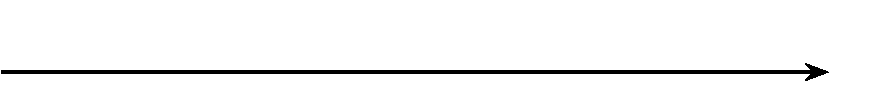
\includegraphics[scale=1]{exist_plain}
			}{
				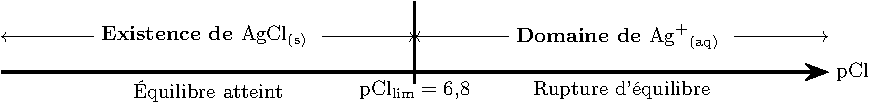
\includegraphics[scale=1]{exist_AgCl-Cl}
			}
			\captionof{figure}{Diagramme d'existence de \ce{AgCl} \protect\pt{1}}
		\end{center}
	}
	\nitem{6}%
	La solubilité de $\ce{AgCl_{\rm(s)}}$ dans l'eau pure est $s\ind{pur} \approx
		\SI{1.3e-5}{mol.L^{-1}}$. Calculer sa solubilité s'il y a déjà $c = \SI{0.1}{mol.L^{-1}}$ de \ce{Cl^-} en solution, et comparer à la situation pure. Comment s'appelle cet effet~? On donne $\pk[s](\ce{AgCl}) = \num{9.8}$.
	\smallbreak
	\psw{
		\noindent
		\begin{isd}
			\psw{
				\begin{enumerate}[label=\sqenumi]
					\item \leavevmode\vspace*{-25pt}\relax
					      \begin{center}
						      \def\rhgt{0.30}
						      \centering
						      \begin{tabularx}{\linewidth}{|l|c||YdYdY|}
							      \hline
							      \multicolumn{2}{|c||}{
								      $\xmathstrut{\rhgt}$
							      \textbf{Équation}\pt{1}} &
							      $\ce{AgCl\sol}$          & $=$                  &
							      $\ce{Ag+\aqu}$           & $+$                  &
							      $\ce{Cl^-\aqu}$                                   \\
							      \hline
							      $\xmathstrut{\rhgt}$
							      Initial                  & $\xi = 0$            &
							      $n$                      & \vline               &
							      $0$                      & \vline               &
							      $cV$                                              \\
							      \hline
							      $\xmathstrut{\rhgt}$
							      Final                    & $\xi_f = \xi_{\equ}$ &
							      $n - \xi_{\equ}$         & \vline               &
							      $\xi_{\equ}$             & \vline               &
							      $cV + \xi_{\equ}$                                 \\
							      \hline
						      \end{tabularx}
					      \end{center}
					      C'est l'\textbf{effet d'ions communs} \pt{1}
				\end{enumerate}
			}
			\tcblower
			\psw{
				\begin{enumerate}[label=\sqenumi, start=2]
					\item \leavevmode\vspace*{-30pt}\relax
					      \begin{gather*}
						      n\ind{dis,max} = \xi\ind{eq} = sV
						      \quad \stm{\Ra} \quad
						      \left\{
						      \begin{array}{rl}
							      [\ce{Ag+}]\ind{eq} & = s
							      \\{}
							      [\ce{Cl-}]\ind{eq} & = \frac{cV + \xi\ind{eq}}{V} = c+s
						      \end{array}
						      \right.
					      \end{gather*}
					\item \leavevmode\vspace*{-33pt}\relax
					      \begin{gather*}
						      K_s \stm{=}
						      % \frac{[\ce{Ag+}]\ind{eq}\times[\ce{Cl-}]\ind{eq}}{{c^\circ}^2} =
						      \frac{s(c+s)}{(c^\circ)^2}
						      % \\\Ra
						      \quad \stackon{$\Lra$}{$s \ll c$} \quad
						      % \beforetext{$s \ll c \Ra$}
						      {c^\circ}^2K_s \approx s \times c
						      \Lra
						      \boxed{s \stm{\approx} \frac{K_s}{c}{c^\circ}^2}
						      \\\Ra
						      \xul{s = \SI{1.8e-9}{mol.L^{-1}}} \pt{1} \ll c \quad
						      \text{\faIcon{check}}
					      \end{gather*}
					      \vspace{-15pt}
				\end{enumerate}
			}
		\end{isd}
	}
	\vfill
	\nitem{3}%
	\leavevmode\vspace*{-20pt}\relax
	\begin{gather*}
		\beforetext{Pour une demi-équation}
		\ce{\alpha Red + \beta H_2O_{\rm(l)} =
		\gamma Ox + \delta {H}^+_{\rm(aq)} + ne^-}
	\end{gather*}
	Donner l'expression du potentiel de \textsc{Nernst} en fonction de la
	température, puis sa forme simplifiée à \SI{25}{\degreeCelsius}.
	\psw{
		\[
			E(\ce{Ox}/\ce{Red}) \stm(un){\stm{=}} E^\circ(\ce{Ox}/\ce{Red}) +
			\frac{RT}{n\Fc} \ln
			\frac{a_{\ce{Ox}}^{\gamma}[\ce{H+}]^{\delta}}
			{a_{\ce{Red}}^{\alpha}{c^\circ}^{\delta}}
			\Ra
			\boxed{
				E(\ce{Ox}/\ce{Red}) \stm{=} E^\circ(\ce{Ox}/\ce{Red}) +
				\frac{\num{0.06}}{n} \log
				\frac{a_{\ce{Ox}}^{\gamma}[\ce{H+}]^{\delta}}
				{a_{\ce{Red}}^{\alpha}{c^\circ}^{\delta}}
			}
		\]
	}
	\nitem{4}%
	Donner les demi-équations puis les potentiels des couples suivants~:
	\smallbreak
	\begin{isd}
		\begin{itemize}
			\item
			      \leftcenters{%
			      $\stm(un){\ce{{Fe}^2+_{\rm(aq)}}}/\ce{Fe_{\rm(s)}}$~:
			      }{%
			      \psw{$\ce{Fe_{\rm(s)} = {Fe}^2+_{\rm(aq)} + 2e^-}$}
			      }
			      \vspace{-15pt}
			      \psw{
				      \[
					      E = E^\circ \left( \ce{Fe^2+}/\ce{Fe} \right) +
					      \frac{\num{0.06}}{2} \log \frac{[\ce{Fe^2+}]}{c^\circ}
				      \]
			      }
			      \vspace{-15pt}
			\item
			      \leftcenters{%
			      $\stm(un){\ce{{Fe}^3+_{\rm(aq)}}}/\ce{{Fe}^2+_{\rm(aq)}}$
			      }{%
			      \psw{$\ce{{Fe}^2+_{\rm(aq)} = {Fe}^3+_{\rm(aq)} + e^-}$}
			      }
			      \vspace{-15pt}
			      \psw{
				      \[
					      E = E^\circ \left( \ce{Fe^3+}/\ce{Fe^2+} \right) +
					      \num{0.06} \log (\frac{[\ce{Fe^3+}]}{[\ce{Fe^2+}]})
				      \]
			      }
			      \vspace{-15pt}
		\end{itemize}
		\tcblower
		\begin{itemize}
			\item $\ce{{MnO_4}^-_{\rm(aq)}/\ce{{Mn}^2+_{\rm(aq)}}}$~: \pt{1}
			      \psw{
				      \begin{gather*}
					      \ce{
					      {Mn}^2+_{\rm(aq)} + 4 H_2O_{\rm(l)}
						      =
						      {MnO_4}^-_{\rm(aq)} + 8 {H}^+_{\rm(aq)} + 5e^-
					      }
					      \\
					      E = E^\circ \left( \ce{{MnO_4}^-/\ce{{Mn}^2+}} \right) +
					      \frac{\num{0.06}}{5}
					      \log ( \frac{[\ce{MnO_4^-}][\ce{H+}]^8}{[\ce{Mn^2+}]{c^\circ}^8})
				      \end{gather*}
			      }
			      \vspace{-15pt}
			\item
			      \leftcenters{%
			      $\stm(un){\ce{{H}^+_{\rm(aq)}/\ce{H_2_{\rm(g)}}}}$
			      }{%
			      \psw{$\ce{H_2_{\rm(g)} = 2 {H}^+_{\rm(aq)} + 2e^-}$}
			      }
			      \vspace{-15pt}
			      \psw{
				      \[
					      E = E^\circ \left( \ce{H+}/\ce{H_2} \right) +
					      \frac{\num{0.06}}{2} \log ( \frac{[\ce{H^+}]^2p^\circ}{{c^\circ}^2p_{\ce{H_2}}})
				      \]
			      }
			      \vspace{-15pt}
		\end{itemize}
	\end{isd}
	\vspace*{-15pt}
	\ifstudent{
		\begin{tikzpicture}[remember picture, overlay]
			\node[anchor=north west, align=left]
			at ([shift={(1.4cm,0)}]current page.north west)
			{\\[5pt]\Large\bfseries Nom~:\\[10pt]\Large\bfseries Prénom~:};
			\node[anchor=north east, align=right]
			at ([shift={(-1.5cm,-17pt)}]current page.north east)
			{\Large\bfseries Note~:\hspace{1cm}/20};
		\end{tikzpicture}
	}
\end{enumerate}
\end{document}
